%*****************************************
\chapter{Data}\label{06:data}
%*****************************************
%TODO Status: pre-draft


\section{Data}\label{intro:TypesOfData}

\begin{wrapfigure}{r}{0.4\textwidth}
	\label{05:fig01} 
	\centering
	
\includegraphics[width=0.4\textwidth]{gfx/06-data} 
\end{wrapfigure}
Data are\footnote{The word ``data'' is plural and is treated that way in this text even though modern usage seems to be trending toward a singular form.} a collection of facts about some topic. As examples, a ``customer loyalty'' program gathers data from customers on how often they shop, what they purchase on each trip, what time of day they typically shop, and all sorts of other data. When data are interpreted in some way they become information. The types of analyses that can be done with data are limited by the types of data involved. The purpose of this chapter is to introduce various concepts about data and show how they can be analyzed.\footnote{Photo by Mika Baumeister on Unsplash}

\subsection{Types of Data}

Psychologist Stanley Smith Stevens defined four generic types of data\cite{stevens1946theory}. Table \ref{tab06.01} summarizes the statistical methods that can be used for the four data types.

\begin{table}[H]
	\centering
	\begin{tabularx}{0.95\linewidth}{p{0.15\linewidth}p{0.40\linewidth}p{0.40\linewidth}}
		\toprule
		\textbf{Type} & \textbf{Central Measure} & \textbf{Statistics} \\
		\midrule
		Nominal & Mode & Chi-square \\
		Ordinal & Median & Percentile \\
		Interval & Arithmetic mean, range, standard deviation & Correlation, regression \\
		Ratio & Geometric mean, harmonic mean & Coefficient of variation \\
		\midrule
		\multicolumn{3}{p{0.95\linewidth}}{Note: All higher-order types can use any of the statistics for the lower order types.} \\	
		\bottomrule
	\end{tabularx}
	\caption{Statistical properties of the data types.}
	\label{tab06.01}
\end{table}

\begin{itemize}
	
	\item \textbf{\Gls{qualitativedata}} groups observations into a limited number of categories; for example, type of pet (cat, dog, bird, etc.) or place of residence (Arizona, California, etc.). Because qualitative data do not have characteristics like means or standard deviations, they are analyzed using non-parametric tests, like Kruskal-Wallis H and Mann-Whitney U. Qualitative data can be further divided into two sub-types, nominal and ordinal.
	
	\begin{itemize}
		\item \textbf{\Gls{nominaldata}} are categories that do not overlap and have no meaningful order, they are merely labels for attributes. Examples of nominal data include occupations (custodial, accounting, sales, etc.) and blood type (A, B, AB, O). A special subcategory of nominal data is binary, or dichotomous, where there are only two possible responses, like ``yes'' and ``no''. Nominal data are sometimes stored in a database using numbers but they cannot be treated like numeric data. For example, binary data, like ``Do you rent or own your home?'' can be stored as ``1 = rent, 2 = own'' but the numbers in this case have no numeric significance and could be replaced by words like ``Rent'' and ``Own.''
		
		\item \textbf{\Gls{ordinaldata}} are categorical data but, unlike nominal, the categories imply some sort of order (which is why it is called ``ordinal'' data). One example of ordinal data is the ``star'' rating system for movies. It is clear that a five-star movie is somehow better than a four-star movie but there is no way to quantify the difference between those two categories. As another example, it is common for hospital staff members to ask patients to rate their pain level on a scale of one to ten. If a patient reports a pain level of ``seven'' but after some sort of treatment later reports a pain level of ``five'' then the pain has clearly decreased but it would be impossible to somehow quantify the exact difference in those two levels. Ordinal scales are most commonly used with Likert-type survey questions where the responses are selections like ``Strongly Agree'', ``Agree'', ``Neutral'', ``Disagree'', ``Strongly Disagree''. Ordinal data are also used when numeric data are grouped. For example, if a dataset included respondents' ages then those numbers could be grouped into categories like ``$ 20-29 $'' and ``$ 30-39 $.'' Those groups would typically be stored in the dataset as a single number so maybe ``$ 2 $'' would represent the ages ``$ 20-29 $,'' which would be ordinal data.
	\end{itemize}
	
	\item \textbf{\Gls{quantitativedata}} are numbers, typically counts or measures, like a person's age, a tree's height, or a truck's weight. Quantitative data are measured with scales that have equal divisions so the difference between any two values can be calculated. Quantitative data are discrete if they are represented by integers, like the count of words in a document, or continuous if they are represented by fractional numbers, like a person's height. Because quantitative data includes characteristics like means and standard deviations, they are analyzed using parametric tests, like T-tests and Analysis of Variance (ANOVA). Quantitative data can be further divided into two sub-types, interval and ratio.
	
	\begin{itemize}
		\item \textbf{\Gls{intervaldata}} use numbers to represent quantities where the distance between any two quantities can be calculated but there is no true zero point on the scale. One example is a temperature scale where the difference between $ 80 $\textdegree and $ 90 $\textdegree is the same as the difference between $ 60 $\textdegree and $ 70 $\textdegree. It is important to note that interval data do not include any sort of true zero point, thus zero degrees Celsius does not mean ``no temperature,'' and without a zero point it is not reasonable to make a statement like $ 20 $\textdegree is twice as hot as $ 10 $\textdegree.
		
		\item \textbf{\Gls{ratiodata}} use numbers to describe a specific measurable distance between two quantities; however, unlike interval data, ratio data have a true zero point. A good example of ratio data is the sales report for an automobile dealership. Because the data are a simple count of the number of automobiles sold it is possible to compare on month with another. Also, since the scale has a true zero point (it is possible to have zero sales) it is possible to state that one month had twice the sales of another.
	\end{itemize}
\end{itemize}

\subsection{Shape of Data}

\subsubsection{About The Normal Distribution (Bell Curve)}

When the quantitative data gathered from some statistical project are plotted on a graph they often form a \gls{normaldistribution} (sometimes called a ``bell curve'' due to its shape). As an example, consider the Scholastic Aptitude Test (SAT) which is administered to more than $ 1.5 $ million high school students every year. Figure \ref{fig06.01} was created with fake data but illustrates the results expected of a typical SAT administration.

\begin{figure}[H]
	\centering
	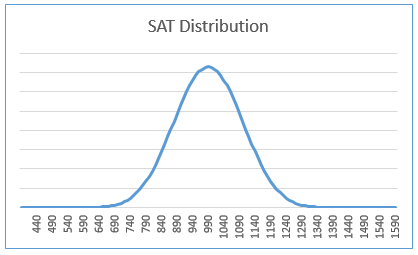
\includegraphics[width=\maxwidth{.95\linewidth}]{gfx/06-SATDistro}
	\caption{Normal Distribution}
	\label{fig06.01}
\end{figure}

SAT scores lie between $ 400 $ and $ 1600 $ as listed across the X-Axis and the number of students who earn each score is plotted. Since the most common score is $ 1000 $ that score is at the peak of the curve. Very few students scored above $ 1300 $ or below $ 650 $ and the curve is near the lower bound beyond those points. This illustrates a normal distribution where most scores are bunched near the center of the graph with only a few at either extreme.

The normal distribution is important because it permits researchers to use specific techniques to test a hypothesis about the sample. For example, perhaps a researcher hypothesized that the graduation rate at university ``A'' was higher than at university ``B'' because students' SAT scores were higher. Since SAT scores have a normal distribution, the researcher could use specific tests, like a t-test, to support or refute the hypothesis. However, if the data were not normally distributed then the researcher would need to use a different group of tests.

\subsubsection{Excess Kurtosis}
One way to mathematically describe a normal distribution is to calculate the length of the tails of a bell curve, and that is called its \gls{excesskurtosis}. For a normal distribution the excess kurtosis is $ 0.00 $, a positive excess kurtosis would indicate longer tails while a negative excess kurtosis would indicate shorter tails. Intuitively, many people believe the excess kurtosis represents the ``peaked-ness'' of the curve since longer tails would tend to lead to a more peaked graph; however, excess kurtosis is a measure of the data outliers, which would be only present in the tails of the graph; so excess kurtosis is not directly indicative of the the ``sharpness'' of the peak. It is difficult to categorically state that some level of excess kurtosis is good or bad. In some cases, data that form a graph with longer tails are desired but in other cases they would be a problem.

Following are three examples of excess kurtosis. Notice that as the excess kurtosis increases the tails become longer. 

\begin{figure}[H]
	\centering
	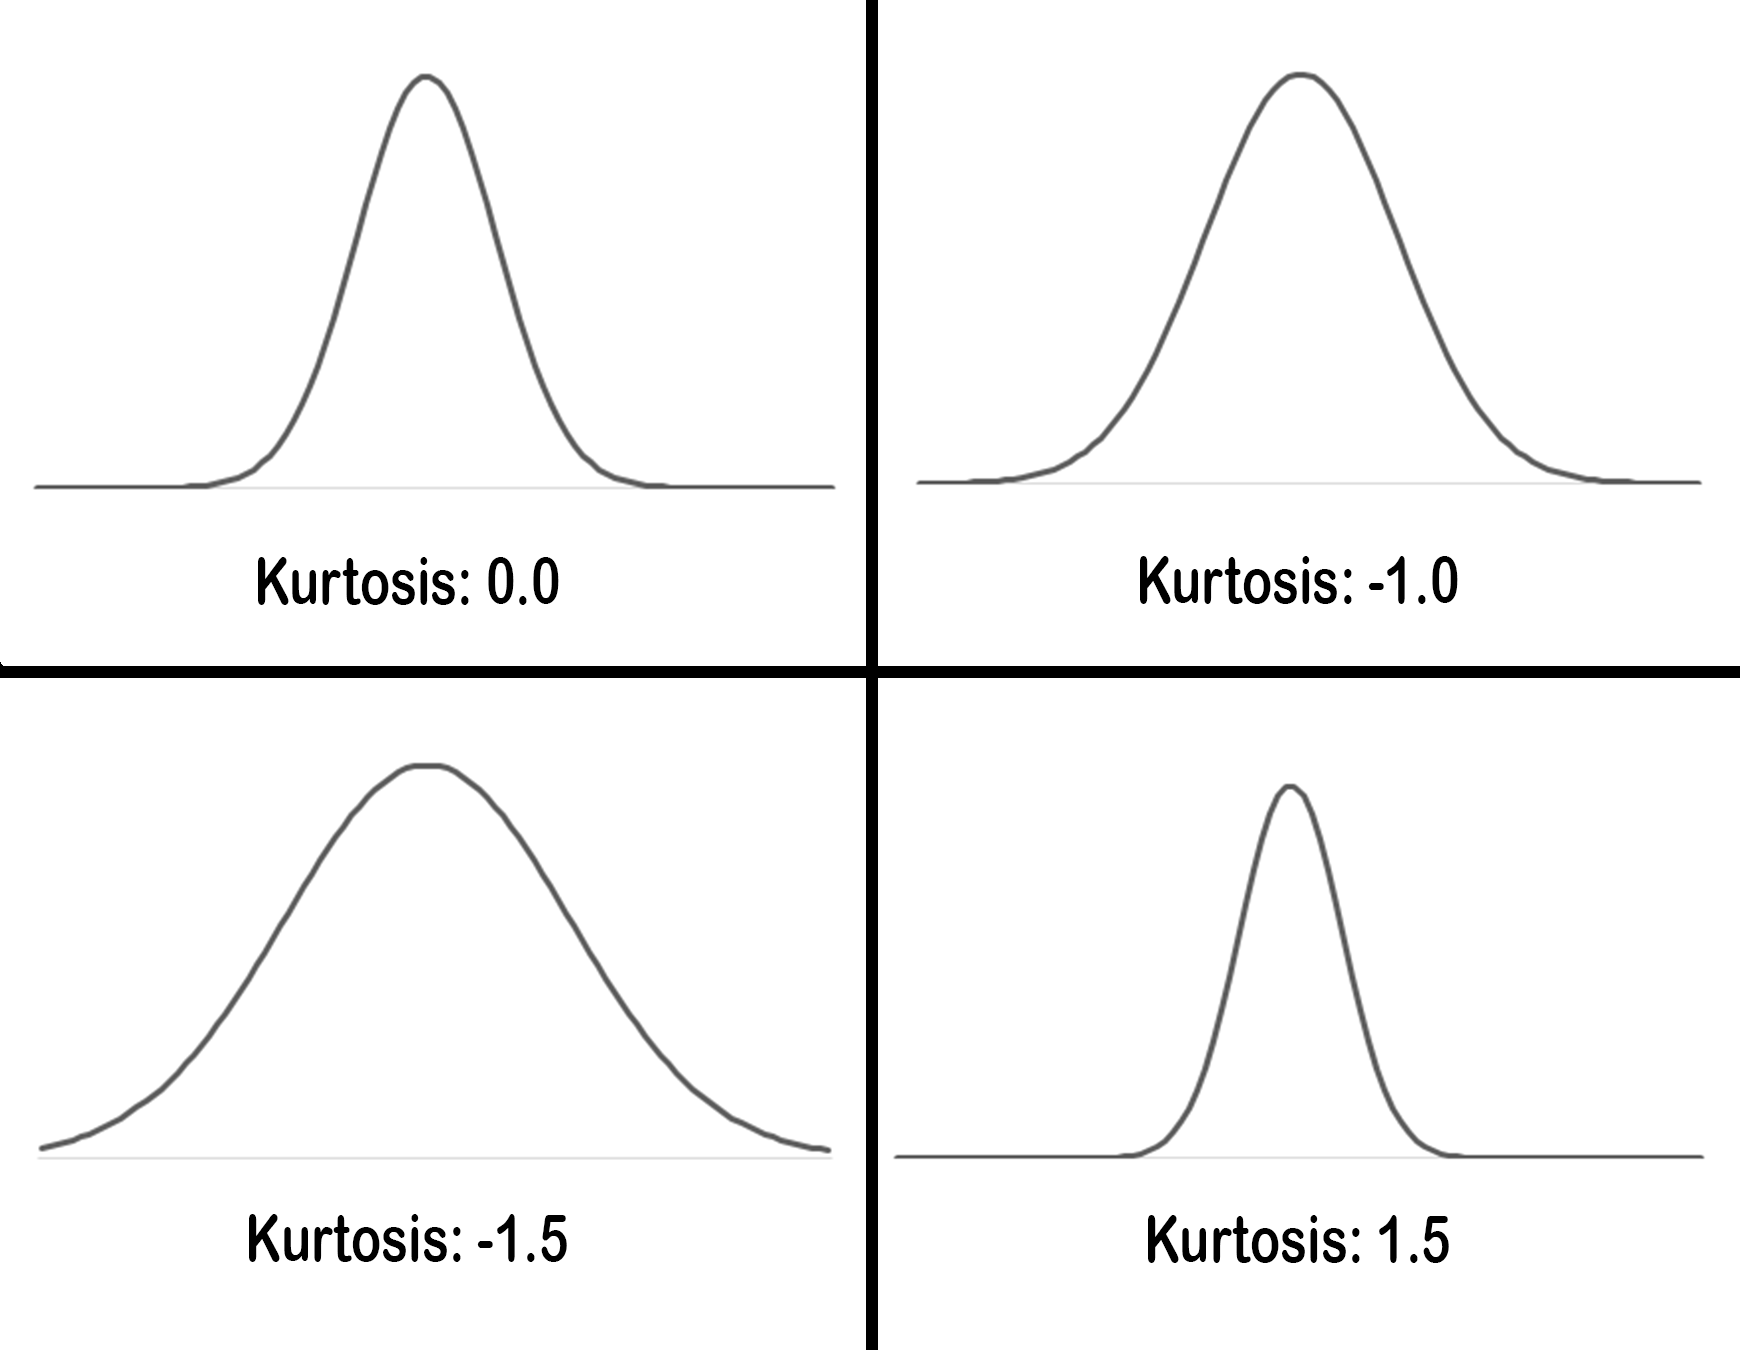
\includegraphics[width=\maxwidth{.95\linewidth}]{gfx/06-Kurtosis}
	\caption{Kurtosis in a Normal Distribution}
	\label{fig06.02}
\end{figure}

\subsubsection{Skew}
The second numerical measure of a normal distribution that is frequently reported is its \gls{skew}, which is a measure of the symmetry of the curve about the mean of the data. The normal distribution in Figure \ref{fig06.03} has a skew of $ 0.00 $. A positive skew indicates that the tail on the right side is longer, which means that there are several data points on the far right side of the graph ``pulling'' the tail out that direction. A negative skew indicates that the tail on the left side of the graph is longer. Following are three examples of skew:

\begin{figure}[H]
	\centering
	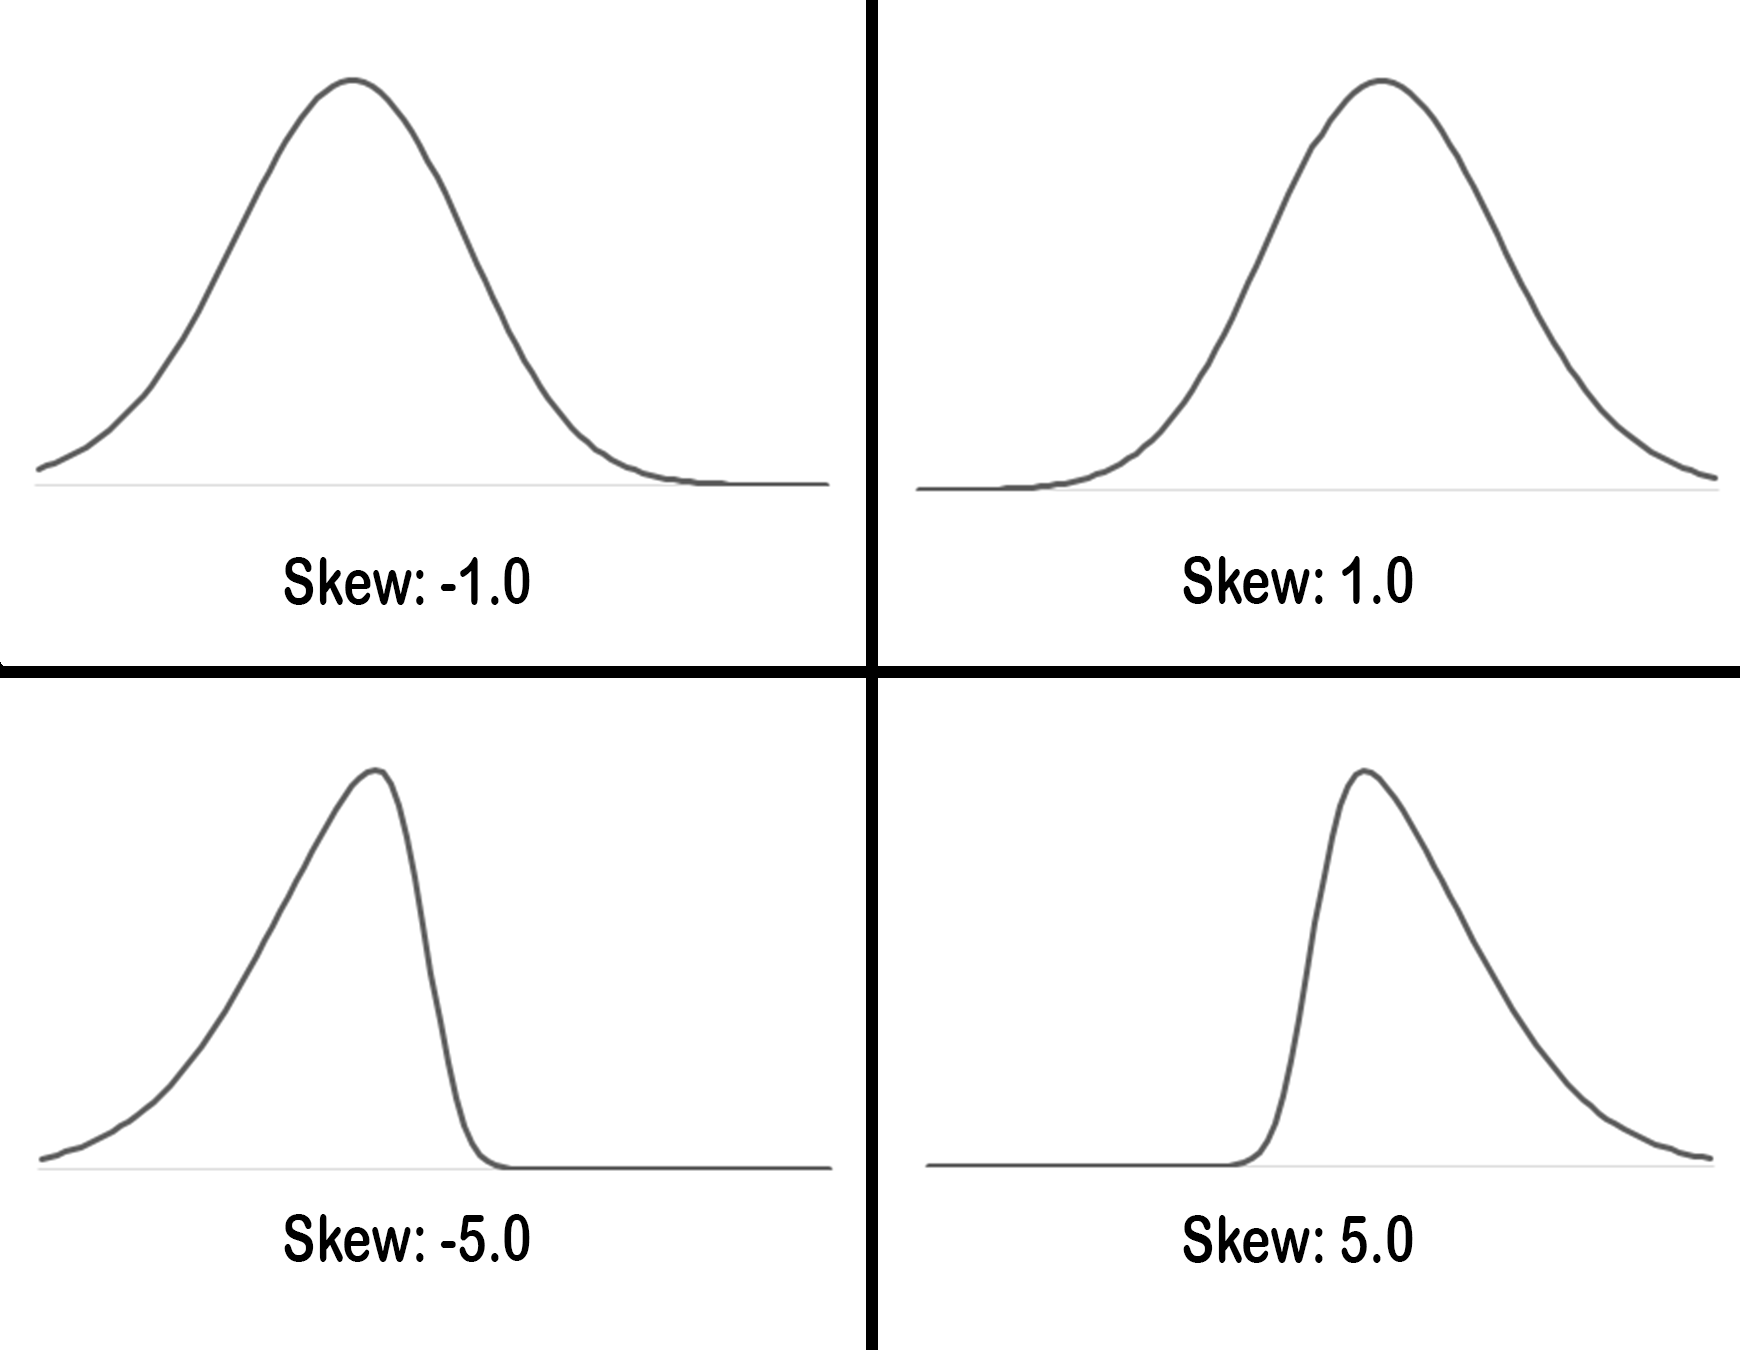
\includegraphics[width=\maxwidth{.95\linewidth}]{gfx/06-Skew}
	\caption{Skew in a Normal Distribution}
	\label{fig06.03}
\end{figure}

\section{Database}

When a lot of data are gathered into a single location they are referred to as a \gls{database}. This is not a new concept. Fifty years ago a library would have a series of 3X5 cards that contained information about all of the books in the library (title, author, subject, etc.). Those cards were stored in a wooden cabinet called the ``card catalog'' and customers could find information about and the location of whatever book they wanted. Today, databases are often contained in electronic form on the internet where they can be accessed from customers' home computers, tablets, or even phones.

Data in a database is typically stored in tables that resemble spreadsheets, that is, rows and columns where each row is one record (or observation) about some phenomenon and each column is one descriptor of that record. For example, a database that contains information about the people who work at a company would be organized such that each row contained data about just one person and each column would contain a single aspect of that person's employment, like name, employee number, date of birth, etc.\footnote{Of course, databases are much more complex than described in this paragraph but this is not a database text so the simple explanation offered is adequate for this context.} A database is designed to deliver answers to questions through a lookup process so, for example, if the CEO of a company wanted to know the birth date for someone in the accounting department that data could be easily found. 

One common problem with any database is ``dirty data.'' These are data that contain errors or are missing. For example, it is easy for a data entry clerk to enter something like ``1000000'' instead of ``100000'' (count the zeros) for a person's salary and create an ``outlier'' in the data. Another common problem are missing data. For example, if employees are asked to update their personal information but someone could not remember their ZIP code then they would simply leave that field blank.

Dirty data makes it difficult to analyze the database. For example, if a researcher wanted to report the median salary for the workers in a factory but ten percent of the salaries were missing from the database then the median would not be accurate. There are several methods statisticians use to mitigate the problems caused by dirty data but those are beyond the scope of this text. 

\subsection{Public Databases}

There are hundreds of publicly available databases that can be used for research. As one example, the United States Census Bureau maintains a huge database that contains information about the people of the United States.\footnote{The US Census Bureau's website is at \url{https://www.census.gov/}.} The data at that site is freely available to anyone who wants to use it, and the site is organized so information is fairly quick and easy to find. As an example, it is not difficult to discover that among adults in the United States, 29\% have a high school diploma, 20\% have a Bachelor's degree, 8\% have a Master's degree, 1.7\% have a Doctoral degree, and the rest fall elsewhere on the education spectrum. The US Census Bureau has more advanced tools available that permit researchers to focus on a single county or even smaller region.

When using a public database, a researcher must be concerned with bias. Since the researcher did not gather the data first-hand it is possible that the data are biased. For example, if the database includes people's attitude towards work how is the researcher going to know if the data gathered was from a well-designed, neutral survey or if it was just gathered using some sort of convenience sample? In general, databases found at governmental websites (with urls that end with .gov) or education websites (with urls that end with .edu) would more likely be bias-free while databases from .com sites would need to have extra attention paid to bias.

Sometimes, students will find a website with a list of links to journal articles or chapters from books. While these are valuable resources for a researcher, they are not the same as a database that contains raw data from a survey, experiment, or other activity. Journal articles provide good information for a literature review but would not be appropriate for an online database source.

\subsection{Using Public Databases}

As an example of using a public database, imagine that the CEO of ``BASVFOODS'' is interested in opening a neighborhood market in a small town they have never serviced before. In order to gather information about that location it is possible to use US Census Bureau data to find out things like the median household size, income, and education level. The CEO could then compare that data with similar data from a town that has a successful store to help inform a decision to open a new store.

\section{Rating Scales}

Researchers must decide on the level of measurement when operationalizing a construct. Rating scales, also called levels of measure, refer to the \textit{values} that an indicator can take, but says nothing about the indicator itself. For example, male, female, and other (or M, F, and O, or $ 1 $, $ 2 $, and $ 3 $) are three rating scales of the indicator ``gender.'' 

Based on the types of \gls{qualitativedata} discussed near the start of this chapter, several different rating scales can be devised and the common ones are binary, Likert, semantic differential, and Guttman. 

\begin{figure}[H]
	\centering
	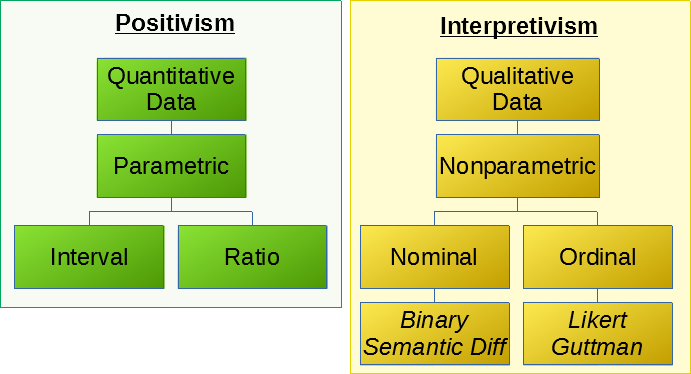
\includegraphics[width=\maxwidth{.95\linewidth}]{gfx/06-DataTypes}
	\caption{Data types}
	\label{fig06.04}
\end{figure}

\begin{description}
	\item[Binary] Binary scales are nominal scales consisting of binary items that assume one of only two possible values, such as yes or no, true or false, and so on. For example, a typical binary scale for a ``political activism'' construct may consist of the six binary items shown in Table \ref{tab06.02}. Each item in this scale is a binary item, and the total number of ``yes'' indicated by a respondent (a value from $ 0 $ to $ 6 $) can be used as an overall measure of that person's political activism. Binary scales can also employ other values, such as male or female for gender, full-time or part-time for employment status, and so forth. If an employment status item is modified to allow for more than two possible values (e.g., unemployed, full-time, part-time, and retired), it is no longer binary, but still remains a nominal scaled item.

	\begin{table}[H]
	\centering
	\begin{tabularx}{0.95\linewidth}{p{0.70\linewidth}p{0.09\linewidth}p{0.09\linewidth}}
		\toprule
		\textbf{Question} & \textbf{Yes} & \textbf{No} \\
		\midrule
		Have you ever written a letter to a public official? & $ \bigcirc $ & $ \bigcirc $ \\ 
		Have you ever signed a political petition? & $ \bigcirc $ & $ \bigcirc $ \\ 
		Have you ever donated money to a political cause? & $ \bigcirc $ & $ \bigcirc $ \\ 
		Have you ever donated money to a candidate running for public office? & $ \bigcirc $ & $ \bigcirc $ \\ 
		Have your ever written a political letter to the editor of a newspaper?& $ \bigcirc $ & $ \bigcirc $ \\ 
		Have you ever persuaded someone to change his/her voting plans? & $ \bigcirc $ & $ \bigcirc $ \\ 
		\bottomrule
	\end{tabularx}
	\caption{Political activism binary scale}
	\label{tab06.02}
	\end{table}
	
	\item[Likert] Designed by Rensis Likert, this is a very popular rating scale for measuring ordinal data in business research. This scale includes Likert items that are simply-worded statements to which respondents can indicate their extent of agreement or disagreement on a five or seven-point scale ranging from ``strongly disagree'' to ``strongly agree.'' A typical example of a six-item Likert scale for the ``employment self-esteem'' construct is shown in table \ref{tab06.03}. Likert scales are summated scales, that is, the overall scale score may be a summation of the attribute values of each item as selected by a respondent.

	\begin{table}[H]
		\centering
		\begin{tabularx}{0.95\linewidth}{p{0.35\linewidth}p{0.10\linewidth}p{0.08\linewidth}p{0.07\linewidth}p{0.07\linewidth}p{0.08\linewidth}}
			\toprule
			{\footnotesize Statement} & {\footnotesize Strongly disagree} & {\footnotesize Disagree} & {\footnotesize Neutral} & {\footnotesize Agree} & {\footnotesize Strongly agree} \\
			\midrule
			{\footnotesize I feel good about my job} & $ \bigcirc $ & $ \bigcirc $ & $ \bigcirc $ & $ \bigcirc $ & $ \bigcirc $ \\
			{\footnotesize I get along well with others at work} & $ \bigcirc $ & $ \bigcirc $ & $ \bigcirc $ & $ \bigcirc $ & $ \bigcirc $ \\
			{\footnotesize I'm proud of my relationship with my supervisor} & $ \bigcirc $ & $ \bigcirc $ & $ \bigcirc $ & $ \bigcirc $ & $ \bigcirc $ \\
			{\footnotesize I feel like I'm making a contribution at work} & $ \bigcirc $ & $ \bigcirc $ & $ \bigcirc $ & $ \bigcirc $ & $ \bigcirc $ \\
			{\footnotesize I can tell that my coworkers respect me} & $ \bigcirc $ & $ \bigcirc $ & $ \bigcirc $ & $ \bigcirc $ & $ \bigcirc $ \\
			\bottomrule
		\end{tabularx}
		\caption{Likert scale for employee self-esteem}
		\label{tab06.03}
	\end{table}
	
	Likert items allow for more granularity (more finely tuned response) than binary items, including whether respondents are neutral to the statement. Three or nine values (often called ``anchors'') may also be used, but it is important to use an odd number of values to allow for a ``neutral'' (or ``neither agree nor disagree'') anchor. Some studies have used a ``forced choice approach'' to force respondents to agree or disagree with the Likert statement by dropping the neutral mid-point and using even number of values, but this is not a good strategy because some people may indeed be neutral to a given statement and the forced choice approach does not provide them the opportunity to record their neutral stance. A key characteristic of a Likert scale is that even though the statements vary in different items or indicators, the anchors (``strongly disagree'' to ``strongly agree'') remain the same. Likert scales are ordinal scales because the anchors are not necessarily equidistant, even though sometimes we treat them like interval scales.
	
	\item[Semantic Differential] This is a composite (multi-item) scale where respondents are asked to indicate their opinions or feelings toward a single statement using different pairs of adjectives framed as polar opposites. For instance, the construct ``attitude toward health insurance'' can be measured using three items shown in Table \ref{tab06.04}. As in the Likert scale, the overall scale score may be a summation of individual item scores. Notice that in Likert scales, the statement changes but the anchors remain the same across items. However, in semantic differential scales, the statement remains constant, while the anchors (adjective pairs) change across items. Semantic differential is believed to be an excellent technique for measuring people's attitude or feelings toward objects, events, or behaviors. 
	
	
	\begin{table}[H]
		\centering
		\begin{tabularx}{0.95\linewidth}{p{0.10\linewidth}p{0.10\linewidth}p{0.10\linewidth}p{0.10\linewidth}p{0.10\linewidth}p{0.10\linewidth}p{0.10\linewidth}}
			\toprule
			\multicolumn{7}{p{0.95\linewidth}}{How would you rate your opinion on health insurance?} \\	
			\midrule
			{} & {\footnotesize Very Much} & {\footnotesize Much} & {\footnotesize Neutral} & {\footnotesize Much} & {\footnotesize Very Much} & {} \\
			\midrule
			{\footnotesize Good} & $ \bigcirc $ & $ \bigcirc $ & $ \bigcirc $ & $ \bigcirc $ & $ \bigcirc $ & {\footnotesize Bad} \\
			{\footnotesize Useful} & $ \bigcirc $ & $ \bigcirc $ & $ \bigcirc $ & $ \bigcirc $ & $ \bigcirc $ & {\footnotesize Useless} \\
			{\footnotesize Caring} & $ \bigcirc $ & $ \bigcirc $ & $ \bigcirc $ & $ \bigcirc $ & $ \bigcirc $ & {\footnotesize Uncaring} \\
			\bottomrule
		\end{tabularx}
		\caption{Semantic differential scale}
		\label{tab06.04}
	\end{table}
	
	\item[Guttman] Designed by Louis Guttman, this composite scale uses a series of items arranged in increasing order of intensity of the construct of interest, from least intense to most intense. As an example, the construct ``attitude toward immigrants'' can be measured using five items shown in Table \ref{tab06.05}. Each item in the Guttman scale has a weight (not indicated above) which varies with the intensity of that item, and the weighted combination of each response is used as aggregate measure of an observation.

	\begin{table}[H]
	\centering
	\begin{tabularx}{0.95\linewidth}{p{0.70\linewidth}p{0.10\linewidth}p{0.10\linewidth}}
		\toprule
		\multicolumn{3}{p{0.95\linewidth}}{How will you rate your opinion on the following statements about immigrants?} \\	
		\midrule
		Do you mind immigrants being citizens of your country? & Yes & No \\
		Do you mind immigrants living in your own neighborhood? & Yes & No \\
		Would you mind living next door to an immigrant? & Yes & No \\
		Would you mind having an immigrant as your close friend? & Yes & No \\
		Would you mind if someone in your family married an immigrant? & Yes & No \\		
		\bottomrule
	\end{tabularx}
	\caption{Guttman scale}
	\label{tab06.05}
	\end{table}
	
\end{description}

\section{Scaling}

The previous section discussed how to measure respondents' responses to predesigned items or indicators belonging to an underlying construct. But how are the indicators themselves created? The process of creating the indicators is called \textit{scaling}. More formally, scaling is a branch of measurement that involves the construction of measures by associating qualitative judgments about unobservable constructs with quantitative, measurable metrics. Stevens\cite{stevens1946theory} said, ``Scaling is the assignment of objects to numbers according to a rule.'' This process of measuring abstract concepts in concrete terms remains one of the most difficult tasks in empirical social science research.

The outcome of a scaling process is a scale, which is a structure for measuring items or indicators of a given construct. Understand that ``scales'', as discussed in this section, are a little different from ``rating scales'' discussed in the previous section. A rating scale is used to capture the respondents' reactions to a given item, for instance, such as a nominal scaled item captures a yes/no reaction and an interval scaled item captures a value between ``strongly disagree'' to ``strongly agree.'' Attaching a rating scale to a statement or instrument is not scaling. Rather, scaling is the formal process of developing scale items, before rating scales can be attached to those items.

Scales can be unidimensional or multidimensional, based on whether the underlying construct is unidimensional (\eg, weight, wind speed, firm size) or multidimensional (\eg, academic aptitude, intelligence). Unidimensional scale measures constructs along a single scale, ranging from high to low. Note that some of these scales may include multiple items, but all of these items attempt to measure the same underlying dimension. This is particularly the case with many social science constructs such as self-esteem, which are assumed to have a single dimension going from low to high. Multi-dimensional scales, on the other hand, employ different items or tests to measure each dimension of the construct separately, and then combine the scores on each dimension to create an overall measure of the construct. For instance, academic aptitude can be measured using two separate tests of students' mathematical and verbal ability and then combining these scores to create an overall measure for academic aptitude. 

Unidimensional scaling methods were developed during the first half of the twentieth century and were named after their creators. The three most popular are: (1) Thurstone's equal-appearing scaling, (2) Likert's summative scaling, and (3) Guttman's cumulative scaling. The three approaches are similar in many respects, with the key differences being the rating of the scale items by judges and the statistical methods used to select the final items.

\subsection{Thurstone's Equal-Appearing Scaling Method}

Louis Thurstone, one of the earliest and most famous scaling theorists, published a scaling method in $ 1925 $\cite{thurstone1925method}. This method starts with a clear conceptual definition of the construct of interest. Based on this definition, potential scale items are generated to measure this construct. These items are generated by experts who know something about the construct being measured. The initial pool of candidate items (ideally $ 80 $ to $ 100 $ items) should be worded in a similar manner, for instance, by framing them as statements to which respondents may agree or disagree (and not as questions or other things). Next, a panel of judges is recruited to select specific items from this candidate pool to represent the construct of interest. Judges may include academics trained in the process of instrument construction or a random sample of respondents of interest (\ie, people who are familiar with the phenomenon). The selection process is done by having each judge independently rate each item on a scale from $ 1 $ to $ 11 $ based on how closely, in their opinion, that item reflects the intended construct ($ 1 $ represents extremely unfavorable and $ 11 $ represents extremely favorable). For each item, the median and inter-quartile range (the difference between the $ 75 $th and the $ 25 $th percentile---a measure of dispersion) would be computed and plotted on a histogram, as shown in Figure 6.1. 

The final scale items are selected as statements that are at equal intervals across a range of medians. This can be done by grouping items with a common median, and then selecting the item with the smallest inter-quartile range within each median group. However, instead of relying entirely on statistical analysis for item selection, a better strategy may be to examine the candidate items at each level and selecting the statement that is the most clear and makes the most sense. The median value of each scale item represents the weight to be used for aggregating the items into a composite scale score representing the construct of interest. We now have a scale which looks like a ruler, with one item or statement at each of the 11 points on the ruler (and weighted as such). Because items appear equally throughout the entire $ 11 $-point range of the scale, this technique is called an equal-appearing scale.

Thurstone also created two additional methods of building unidimensional scales---the method of successive intervals and the method of paired comparisons---which are both very similar to the method of equal-appearing intervals, except for how judges are asked to rate the data. For instance, the method of paired comparison requires each judge to make a judgment between each pair of statements (rather than rate each statement independently on a $ 1 $ to $ 11 $ scale). Hence, the name paired comparison method. With a lot of statements, this approach can be enormously time consuming and unwieldy compared to the method of equal-appearing intervals.

\subsection{Likert's Summative Scaling Method}

The Likert method, a unidimensional scaling method developed by Murphy and Likert (1938), is quite possibly the most popular of the three scaling approaches described in this chapter. As with Thurstone's method, the Likert method also starts with a clear definition of the construct of interest, and using a set of experts to generate about $ 80 $ to $ 100 $ potential scale items. These items are then rated by judges on a $ 1 $ to $ 5 $ (or $ 1 $ to $ 7 $) rating scale as follows: $ 1 $ for strongly disagree with the concept, $ 2 $ for somewhat disagree with the concept, $ 3 $ for undecided, $ 4 $ for somewhat agree with the concept, and $ 5 $ for strongly agree with the concept. Following this rating, specific items can be selected for the final scale can be selected in one of several ways: ($ 1 $) by computing bivariate correlations between judges rating of each item and the total item (created by summing all individual items for each respondent), and throwing out items with low (\eg, less than $ 0.60 $) item-to-total correlations, or ($ 2 $) by averaging the rating for each item for the top quartile and the bottom quartile of judges, doing a t-test for the difference in means, and selecting items that have high t-values (i.e., those that discriminates best between the top and bottom quartile responses). In the end, researcher's judgment may be used to obtain a relatively small (say $ 10 $ to $ 15 $) set of items that have high item-to-total correlations and high discrimination (\ie, high t-values). The Likert method assumes equal weights for all items, and hence, respondent's responses to each item can be summed to create a composite score for that respondent. Hence, this method is called a summated scale. Note that any item with reversed meaning from the original direction of the construct must be reverse coded (i.e., $ 1 $ becomes a $ 5 $, $ 2 $ becomes a $ 4 $, and so forth) before summating.

\subsection{Guttman's cumulative scaling method}

Designed by Guttman (1950), the cumulative scaling method is based on Emory Bogardus' social distance technique, which assumes that people's willingness to participate in social relations with other people vary in degrees of intensity, and measures that intensity using a list of items arranged from ``least intense'' to ``most intense''. The idea is that people who agree with one item on this list also agree with all previous items. In practice, we seldom find a set of items that matches this cumulative pattern perfectly. A scalogram analysis is used to examine how closely a set of items corresponds to the idea of cumulativeness.

Like previous scaling methods, the Guttman method also starts with a clear definition of the construct of interest, and then using experts to develop a large set of candidate items. A group of judges then rate each candidate item as ``yes'' if they view the item as being favorable to the construct and ``no'' if they see the item as unfavorable. Next, a matrix or table is created showing the judges' responses to all candidate items. This matrix is sorted in decreasing order from judges with more ``yes'' at the top to those with fewer ``yes'' at the bottom. Judges with the same number of ``yes'', the statements can be sorted from left to right based on most number of agreements to least. The resulting matrix will resemble Table 6.6. Notice that the scale is now almost cumulative when read from left to right (across the items). However, there may be a few exceptions, as shown in Table 6.6, and hence the scale is not entirely cumulative. To determine a set of items that best approximates the cumulativeness property, a data analysis technique called scalogram analysis can be used (or this can be done visually if the number of items is small). The statistical technique also estimates a score for each item that can be used to compute a respondent's overall score on the entire set of items.

\section{Indexes}

An index is a composite score derived from aggregating measures of multiple constructs (called components) using a set of rules and formulas. It is different from scales in that scales also aggregate measures, but these measures measure different dimensions or the same dimension of a single construct. A well-known example of an index is the \gls{cpi}, which is computed every month by the Bureau of Labor Statistics of the U.S. Department of Labor. The \gls{cpi} is a measure of how much consumers have to pay for goods and services in general, and is divided into eight major categories (food and beverages, housing, apparel, transportation, healthcare, recreation, education and communication, and ``other goods and services''), which are further subdivided into more than $ 200 $ smaller items. Each month, government employees call all over the country to get the current prices of more than $ 80,000 $ items. Using a complicated weighting scheme that takes into account the location and probability of purchase of each item, these prices are combined by analysts, which are then combined into an overall index score using a series of formulas and rules.

Another example of index is \gls{ses}, also called the Duncan socioeconomic index (SEI). This index is a combination of three constructs: income, education, and occupation. Income is measured in dollars, education in years or degrees achieved, and occupation is classified into categories or levels by status. These very different measures are combined to create an overall SES index score, using a weighted combination of ``occupational education'' (percentage of people in that occupation who had one or more year of college education) and ``occupational income'' (percentage of people in that occupation who earned more than a specific annual income). However, SES index measurement has generated a lot of controversy and disagreement among researchers.

The process of creating an index is similar to that of a scale. First, conceptualize (define) the index and its constituent components. Though this appears simple, there may be a lot of disagreement among judges on what components (constructs) should be included or excluded from an index. For instance, in the SES index, isn't income correlated with education and occupation, and if so, should we include one component only or all three components? Reviewing the literature, using theories, and/or interviewing experts or key stakeholders may help resolve this issue. Second, operationalize and measure each component. For instance, how will you categorize occupations, particularly since some occupations may have changed with time (e.g., there were no Web developers before the Internet). Third, create a rule or formula for calculating the index score. Again, this process may involve a lot of subjectivity. Lastly, validate the index score using existing or new data.

Though indexes and scales yield a single numerical score or value representing a construct of interest, they are different in many ways. First, indexes often comprise of components that are very different from each other (e.g., income, education, and occupation in the \gls{ses} index) and are measured in different ways. However, scales typically involve a set of similar items that use the same rating scale (such as a five-point Likert scale). Second, indexes often combine objectively measurable values such as prices or income, while scales are designed to assess subjective or judgmental constructs such as attitude, prejudice, or self-esteem. Some argue that the sophistication of the scaling methodology makes scales different from indexes, while others suggest that indexing methodology can be equally sophisticated. Nevertheless, indexes and scales are both essential tools in social science research.

\section{Typologies}

Scales and indexes generate ordinal measures of unidimensional constructs. However, researchers sometimes wish to summarize measures of two or more constructs to create a set of categories or types called a typology. Unlike scales or indexes, typologies are multidimensional but include only nominal variables. For instance, one can create a political typology of newspapers based on their orientation toward domestic and foreign policy, as expressed in their editorial columns, as shown in Figure 6.2. This typology can be used to categorize newspapers into one of four ``ideal types'' (A through D), identify the distribution of newspapers across these ideal types, and perhaps even create a classification model to classifying newspapers into one of these four ideal types depending on other attributes.

\section{Statistical Tests}

Once the data are gathered it is important to run some statistical processes to see if the data contains anything of interest. While there are hundreds of tests that can be used, here is a bit of information about the most common tests.

\subsection{Central Measures}

\subsection{Dispersion}

\subsection{Frequency Tables}

\subsection{Correlation}

\subsection{Parametric Hypothesis Tests}

\subsection{Nonparametric Hypothesis Tests}

\subsection{Data Mining}

\subsubsection{K-Means Clusters}

\subsubsection{Decision Tree}

\begin{figure}[H]
	\centering
	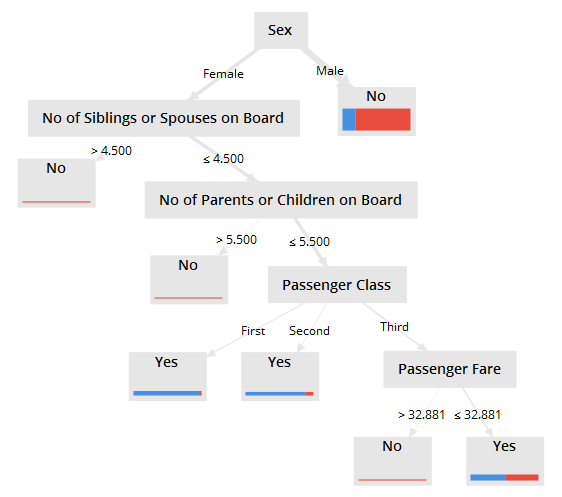
\includegraphics[width=\maxwidth{.95\linewidth}]{gfx/06-DecisionTree}
	\caption{Decision Tree}
	\label{fig06.05}
\end{figure}




\subsubsection{Market Basket}

\begin{figure}[H]
	\centering
	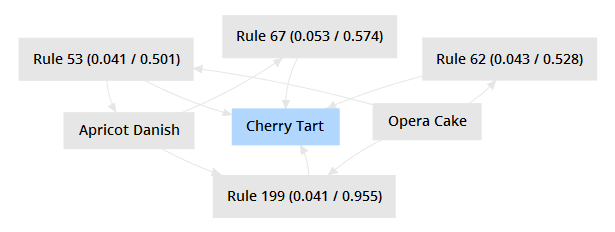
\includegraphics[width=\maxwidth{.95\linewidth}]{gfx/06-MarketBasketGraph}
	\caption{Market Basket Graph}
	\label{fig06.06}
\end{figure}


\begin{figure}[H]
	\centering
	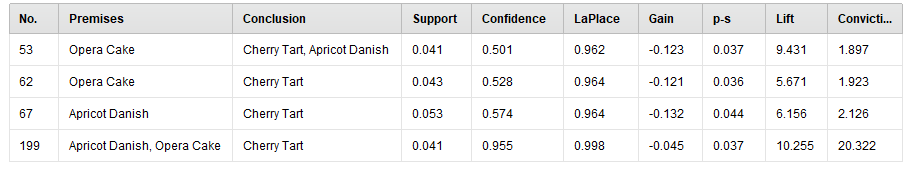
\includegraphics[width=\maxwidth{.95\linewidth}]{gfx/06-MarketBasketRules}
	\caption{Market Basket Rules}
	\label{fig06.07}
\end{figure}


\section{Summary}\label{ch06:summary}

Lorem ipsum dolor sit amet, consectetuer adipiscing elit. Aenean commodo ligula eget dolor. Aenean massa. Cum sociis natoque penatibus et
